\begin{figure}
	\centering
	\subfigure[$\Delta t$ = 6 horas]{
	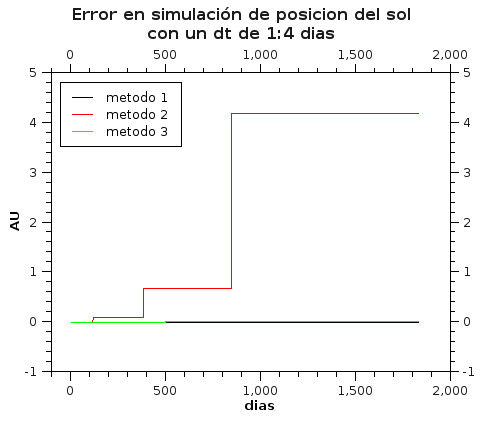
\includegraphics[scale=0.40]{img/ej1/error/error_sol_4.png}
	\label{fig:ej1_err_sol_4}
	}
	\subfigure[$\Delta t$ = 1 hora]{
	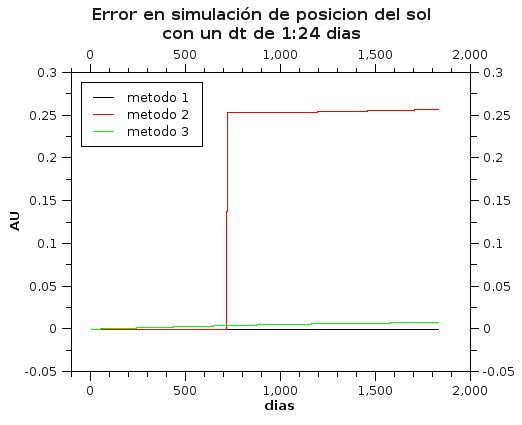
\includegraphics[scale=0.40]{img/ej1/error/error_sol_24.png}
	\label{fig:ej1_err_sol_24}
	}
	\\
	\subfigure[$\Delta t$ = 6 horas]{
	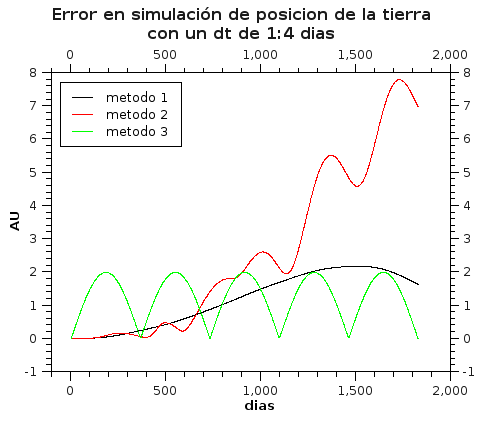
\includegraphics[scale=0.40]{img/ej1/error/error_tierra_4.png}
	\label{fig:ej1_err_tierra_4}
	}
	\subfigure[$\Delta t$ = 1 hora]{
	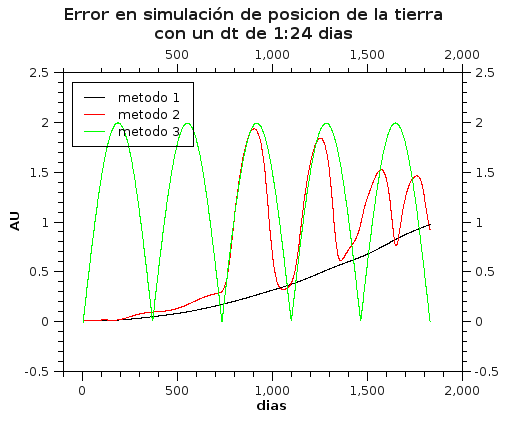
\includegraphics[scale=0.40]{img/ej1/error/error_tierra_24.png}
	\label{fig:ej1_err_tierra_24}
	}
	\\
	\subfigure[$\Delta t$ = 6 horas]{
	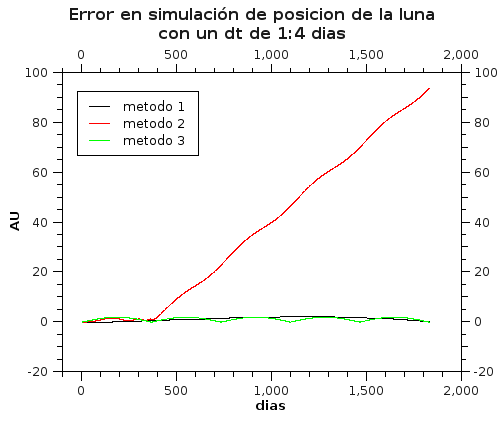
\includegraphics[scale=0.40]{img/ej1/error/error_luna_4.png}
	\label{fig:ej1_err_luna_4}
	}
	\subfigure[$\Delta t$ = 1 hora]{
	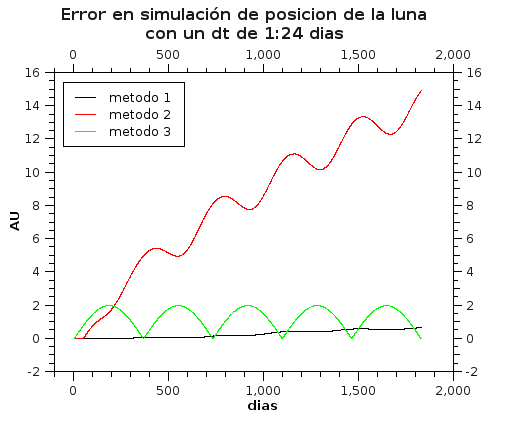
\includegraphics[scale=0.40]{img/ej1/error/error_luna_24.png}
	\label{fig:ej1_err_luna_24}
	}
	\caption{
		Errores de las posiciónes simuladas de los cuerpos sol, tierra y luna,
		con respecto a los datos de la NASA en función del tiempo.
		El período de simulación es de 5 años.
	}
	\label{ fig:res_ej1_err }
\end{figure}
